\chapter{Исследовательский раздел}

В данном разделе будут представлены замеры времени работы реализаций алгоритмов.

\section{Технические характеристики}

Технические характеристики устройства, на котором выполнялось тестирование представлены далее.

\begin{itemize}
    \item Операционная система: macOS Catalina версия 10.15.6;
    \item Память: 8 GB 1600 MHz DDR3;
    \item Процессор: 1,8 GHz 2‑ядерный процессор Intel Core i5.
\end{itemize}

Тестирование проводилось на ноутбуке, включенном в сеть электропитания.
Во время тестирования ноутбук был нагружен только встроенными приложениями окружения рабочего стола.

\section{Сравнительный анализ на основе замеров времени работы алгоритмов}

Был проведен замер времени работы каждого из алгоритмов с помощью функции process\_time(), которая находится в модуле time языка Python.
Для сравнения алгоритмов перемножения матриц используются квадратные матрицы четных и нечетных размерностей. Замеры времени усреднялись, для каждого алгоритма проводилось по 3 итерации. \\

Примем за лучший случай четную размерность, а за худший - нечетную.

\begin{table}[H]
	\centering
	\caption{Временные замеры работы алгоритмов для лучшего случая}
	\begin{tabular}{c|c|c|c|c|c|c|c|c|c}
		\text{Количество} & \text{Простой} & \text{Виноград} & \text{Виноград с оптимизациями}\\
		\hline
		100 & 0.42 & 0.34 & 0.28\\
        200 & 2.82 & 2.81 & 2.28\\
        350 & 9.26 & 9.81 & 7.81\\
        400 & 22.67 & 24.25 & 19.05\\
        500 & 42.26 & 48.95 & 38.01\\

	\end{tabular}
\end{table}

\begin{table}[H]
	\centering
	\caption{Временные замеры работы алгоритмов для худшего случая}
	\begin{tabular}{c|c|c|c|c|c|c|c|c|c}
		\text{Количество} & \text{Простой} & \text{Виноград} & \text{Виноград с оптимизациями}\\
		\hline
        101 & 0.30 & 0.36 & 0.29\\
        201 & 2.44 & 2.88 & 2.39\\
        301 & 8.74 & 10.07 & 7.93\\
        401 & 21.16 & 24.43 & 19.51\\
        501 & 41.33 & 49.17 & 38.61\\
	\end{tabular}
\end{table}

\begin{figure}[H]
	\centering
	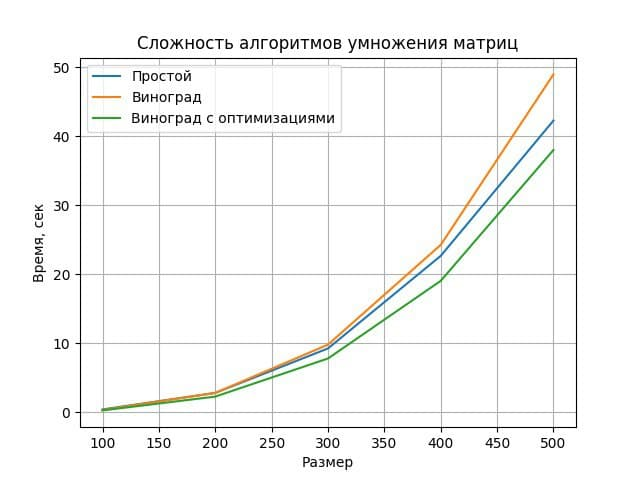
\includegraphics[scale = 0.7]{assets/ls.jpg}
	\caption{Время работы алгоритмов для лучшего случая}
	\label{fig:plot_sorted}
\end{figure}

\begin{figure}[H]
	\centering
	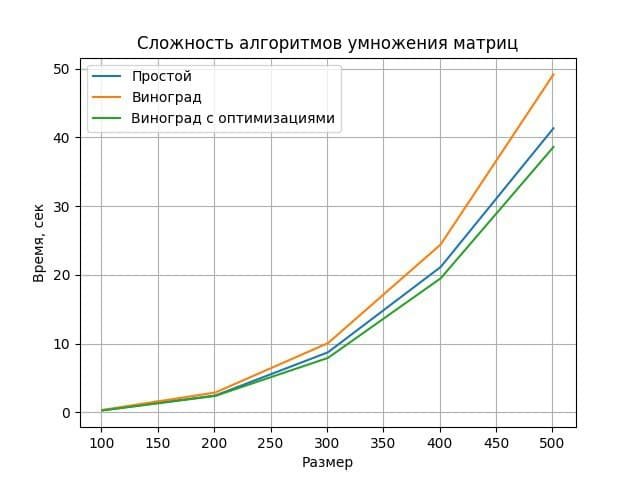
\includegraphics[scale = 0.7]{assets/hs.jpg}
	\caption{Время работы алгоритмов для худшего случая}
	\label{fig:plot_sorted}
\end{figure}

\section{Вывод}


В данном разделе было произведено сравнение количества затраченного времени вышеизложенных алгоритмов.

Исходя из полученных результатов, можно сделать вывод, что простой алгоритм и алгоритм винограда (без оптимизаций) работают приблизительно одинаково, но на графиках мы получили, что простой алгоритм работает чуть быстрее (±7 сек), возможно, это произошло из-за особенностей языка Python, но в любом случае алгоритм винограда следует применять только при очень больших размерностях матриц. Так же мы видим, что виноград с оптимизациями работает быстрее всех алгоритмов на лучших и худших случаях ±5 сек.
